% Generated by Sphinx.
\def\sphinxdocclass{report}
\documentclass[letterpaper,10pt,english]{sphinxmanual}
\usepackage[utf8]{inputenc}
\DeclareUnicodeCharacter{00A0}{\nobreakspace}
\usepackage{cmap}
\usepackage[T1]{fontenc}
\usepackage{babel}
\usepackage{times}
\usepackage[Bjarne]{fncychap}
\usepackage{longtable}
\usepackage{sphinx}
\usepackage{multirow}


\title{python-shop-sdk Documentation}
\date{March 28, 2014}
\release{0.1}
\author{Arne Simon =\textgreater{} email::{[}arne.simon@slice-dice.de{]}}
\newcommand{\sphinxlogo}{}
\renewcommand{\releasename}{Release}
\makeindex

\makeatletter
\def\PYG@reset{\let\PYG@it=\relax \let\PYG@bf=\relax%
    \let\PYG@ul=\relax \let\PYG@tc=\relax%
    \let\PYG@bc=\relax \let\PYG@ff=\relax}
\def\PYG@tok#1{\csname PYG@tok@#1\endcsname}
\def\PYG@toks#1+{\ifx\relax#1\empty\else%
    \PYG@tok{#1}\expandafter\PYG@toks\fi}
\def\PYG@do#1{\PYG@bc{\PYG@tc{\PYG@ul{%
    \PYG@it{\PYG@bf{\PYG@ff{#1}}}}}}}
\def\PYG#1#2{\PYG@reset\PYG@toks#1+\relax+\PYG@do{#2}}

\expandafter\def\csname PYG@tok@gd\endcsname{\def\PYG@tc##1{\textcolor[rgb]{0.63,0.00,0.00}{##1}}}
\expandafter\def\csname PYG@tok@gu\endcsname{\let\PYG@bf=\textbf\def\PYG@tc##1{\textcolor[rgb]{0.50,0.00,0.50}{##1}}}
\expandafter\def\csname PYG@tok@gt\endcsname{\def\PYG@tc##1{\textcolor[rgb]{0.00,0.27,0.87}{##1}}}
\expandafter\def\csname PYG@tok@gs\endcsname{\let\PYG@bf=\textbf}
\expandafter\def\csname PYG@tok@gr\endcsname{\def\PYG@tc##1{\textcolor[rgb]{1.00,0.00,0.00}{##1}}}
\expandafter\def\csname PYG@tok@cm\endcsname{\let\PYG@it=\textit\def\PYG@tc##1{\textcolor[rgb]{0.25,0.50,0.56}{##1}}}
\expandafter\def\csname PYG@tok@vg\endcsname{\def\PYG@tc##1{\textcolor[rgb]{0.73,0.38,0.84}{##1}}}
\expandafter\def\csname PYG@tok@m\endcsname{\def\PYG@tc##1{\textcolor[rgb]{0.13,0.50,0.31}{##1}}}
\expandafter\def\csname PYG@tok@mh\endcsname{\def\PYG@tc##1{\textcolor[rgb]{0.13,0.50,0.31}{##1}}}
\expandafter\def\csname PYG@tok@cs\endcsname{\def\PYG@tc##1{\textcolor[rgb]{0.25,0.50,0.56}{##1}}\def\PYG@bc##1{\setlength{\fboxsep}{0pt}\colorbox[rgb]{1.00,0.94,0.94}{\strut ##1}}}
\expandafter\def\csname PYG@tok@ge\endcsname{\let\PYG@it=\textit}
\expandafter\def\csname PYG@tok@vc\endcsname{\def\PYG@tc##1{\textcolor[rgb]{0.73,0.38,0.84}{##1}}}
\expandafter\def\csname PYG@tok@il\endcsname{\def\PYG@tc##1{\textcolor[rgb]{0.13,0.50,0.31}{##1}}}
\expandafter\def\csname PYG@tok@go\endcsname{\def\PYG@tc##1{\textcolor[rgb]{0.20,0.20,0.20}{##1}}}
\expandafter\def\csname PYG@tok@cp\endcsname{\def\PYG@tc##1{\textcolor[rgb]{0.00,0.44,0.13}{##1}}}
\expandafter\def\csname PYG@tok@gi\endcsname{\def\PYG@tc##1{\textcolor[rgb]{0.00,0.63,0.00}{##1}}}
\expandafter\def\csname PYG@tok@gh\endcsname{\let\PYG@bf=\textbf\def\PYG@tc##1{\textcolor[rgb]{0.00,0.00,0.50}{##1}}}
\expandafter\def\csname PYG@tok@ni\endcsname{\let\PYG@bf=\textbf\def\PYG@tc##1{\textcolor[rgb]{0.84,0.33,0.22}{##1}}}
\expandafter\def\csname PYG@tok@nl\endcsname{\let\PYG@bf=\textbf\def\PYG@tc##1{\textcolor[rgb]{0.00,0.13,0.44}{##1}}}
\expandafter\def\csname PYG@tok@nn\endcsname{\let\PYG@bf=\textbf\def\PYG@tc##1{\textcolor[rgb]{0.05,0.52,0.71}{##1}}}
\expandafter\def\csname PYG@tok@no\endcsname{\def\PYG@tc##1{\textcolor[rgb]{0.38,0.68,0.84}{##1}}}
\expandafter\def\csname PYG@tok@na\endcsname{\def\PYG@tc##1{\textcolor[rgb]{0.25,0.44,0.63}{##1}}}
\expandafter\def\csname PYG@tok@nb\endcsname{\def\PYG@tc##1{\textcolor[rgb]{0.00,0.44,0.13}{##1}}}
\expandafter\def\csname PYG@tok@nc\endcsname{\let\PYG@bf=\textbf\def\PYG@tc##1{\textcolor[rgb]{0.05,0.52,0.71}{##1}}}
\expandafter\def\csname PYG@tok@nd\endcsname{\let\PYG@bf=\textbf\def\PYG@tc##1{\textcolor[rgb]{0.33,0.33,0.33}{##1}}}
\expandafter\def\csname PYG@tok@ne\endcsname{\def\PYG@tc##1{\textcolor[rgb]{0.00,0.44,0.13}{##1}}}
\expandafter\def\csname PYG@tok@nf\endcsname{\def\PYG@tc##1{\textcolor[rgb]{0.02,0.16,0.49}{##1}}}
\expandafter\def\csname PYG@tok@si\endcsname{\let\PYG@it=\textit\def\PYG@tc##1{\textcolor[rgb]{0.44,0.63,0.82}{##1}}}
\expandafter\def\csname PYG@tok@s2\endcsname{\def\PYG@tc##1{\textcolor[rgb]{0.25,0.44,0.63}{##1}}}
\expandafter\def\csname PYG@tok@vi\endcsname{\def\PYG@tc##1{\textcolor[rgb]{0.73,0.38,0.84}{##1}}}
\expandafter\def\csname PYG@tok@nt\endcsname{\let\PYG@bf=\textbf\def\PYG@tc##1{\textcolor[rgb]{0.02,0.16,0.45}{##1}}}
\expandafter\def\csname PYG@tok@nv\endcsname{\def\PYG@tc##1{\textcolor[rgb]{0.73,0.38,0.84}{##1}}}
\expandafter\def\csname PYG@tok@s1\endcsname{\def\PYG@tc##1{\textcolor[rgb]{0.25,0.44,0.63}{##1}}}
\expandafter\def\csname PYG@tok@gp\endcsname{\let\PYG@bf=\textbf\def\PYG@tc##1{\textcolor[rgb]{0.78,0.36,0.04}{##1}}}
\expandafter\def\csname PYG@tok@sh\endcsname{\def\PYG@tc##1{\textcolor[rgb]{0.25,0.44,0.63}{##1}}}
\expandafter\def\csname PYG@tok@ow\endcsname{\let\PYG@bf=\textbf\def\PYG@tc##1{\textcolor[rgb]{0.00,0.44,0.13}{##1}}}
\expandafter\def\csname PYG@tok@sx\endcsname{\def\PYG@tc##1{\textcolor[rgb]{0.78,0.36,0.04}{##1}}}
\expandafter\def\csname PYG@tok@bp\endcsname{\def\PYG@tc##1{\textcolor[rgb]{0.00,0.44,0.13}{##1}}}
\expandafter\def\csname PYG@tok@c1\endcsname{\let\PYG@it=\textit\def\PYG@tc##1{\textcolor[rgb]{0.25,0.50,0.56}{##1}}}
\expandafter\def\csname PYG@tok@kc\endcsname{\let\PYG@bf=\textbf\def\PYG@tc##1{\textcolor[rgb]{0.00,0.44,0.13}{##1}}}
\expandafter\def\csname PYG@tok@c\endcsname{\let\PYG@it=\textit\def\PYG@tc##1{\textcolor[rgb]{0.25,0.50,0.56}{##1}}}
\expandafter\def\csname PYG@tok@mf\endcsname{\def\PYG@tc##1{\textcolor[rgb]{0.13,0.50,0.31}{##1}}}
\expandafter\def\csname PYG@tok@err\endcsname{\def\PYG@bc##1{\setlength{\fboxsep}{0pt}\fcolorbox[rgb]{1.00,0.00,0.00}{1,1,1}{\strut ##1}}}
\expandafter\def\csname PYG@tok@kd\endcsname{\let\PYG@bf=\textbf\def\PYG@tc##1{\textcolor[rgb]{0.00,0.44,0.13}{##1}}}
\expandafter\def\csname PYG@tok@ss\endcsname{\def\PYG@tc##1{\textcolor[rgb]{0.32,0.47,0.09}{##1}}}
\expandafter\def\csname PYG@tok@sr\endcsname{\def\PYG@tc##1{\textcolor[rgb]{0.14,0.33,0.53}{##1}}}
\expandafter\def\csname PYG@tok@mo\endcsname{\def\PYG@tc##1{\textcolor[rgb]{0.13,0.50,0.31}{##1}}}
\expandafter\def\csname PYG@tok@mi\endcsname{\def\PYG@tc##1{\textcolor[rgb]{0.13,0.50,0.31}{##1}}}
\expandafter\def\csname PYG@tok@kn\endcsname{\let\PYG@bf=\textbf\def\PYG@tc##1{\textcolor[rgb]{0.00,0.44,0.13}{##1}}}
\expandafter\def\csname PYG@tok@o\endcsname{\def\PYG@tc##1{\textcolor[rgb]{0.40,0.40,0.40}{##1}}}
\expandafter\def\csname PYG@tok@kr\endcsname{\let\PYG@bf=\textbf\def\PYG@tc##1{\textcolor[rgb]{0.00,0.44,0.13}{##1}}}
\expandafter\def\csname PYG@tok@s\endcsname{\def\PYG@tc##1{\textcolor[rgb]{0.25,0.44,0.63}{##1}}}
\expandafter\def\csname PYG@tok@kp\endcsname{\def\PYG@tc##1{\textcolor[rgb]{0.00,0.44,0.13}{##1}}}
\expandafter\def\csname PYG@tok@w\endcsname{\def\PYG@tc##1{\textcolor[rgb]{0.73,0.73,0.73}{##1}}}
\expandafter\def\csname PYG@tok@kt\endcsname{\def\PYG@tc##1{\textcolor[rgb]{0.56,0.13,0.00}{##1}}}
\expandafter\def\csname PYG@tok@sc\endcsname{\def\PYG@tc##1{\textcolor[rgb]{0.25,0.44,0.63}{##1}}}
\expandafter\def\csname PYG@tok@sb\endcsname{\def\PYG@tc##1{\textcolor[rgb]{0.25,0.44,0.63}{##1}}}
\expandafter\def\csname PYG@tok@k\endcsname{\let\PYG@bf=\textbf\def\PYG@tc##1{\textcolor[rgb]{0.00,0.44,0.13}{##1}}}
\expandafter\def\csname PYG@tok@se\endcsname{\let\PYG@bf=\textbf\def\PYG@tc##1{\textcolor[rgb]{0.25,0.44,0.63}{##1}}}
\expandafter\def\csname PYG@tok@sd\endcsname{\let\PYG@it=\textit\def\PYG@tc##1{\textcolor[rgb]{0.25,0.44,0.63}{##1}}}

\def\PYGZbs{\char`\\}
\def\PYGZus{\char`\_}
\def\PYGZob{\char`\{}
\def\PYGZcb{\char`\}}
\def\PYGZca{\char`\^}
\def\PYGZam{\char`\&}
\def\PYGZlt{\char`\<}
\def\PYGZgt{\char`\>}
\def\PYGZsh{\char`\#}
\def\PYGZpc{\char`\%}
\def\PYGZdl{\char`\$}
\def\PYGZhy{\char`\-}
\def\PYGZsq{\char`\'}
\def\PYGZdq{\char`\"}
\def\PYGZti{\char`\~}
% for compatibility with earlier versions
\def\PYGZat{@}
\def\PYGZlb{[}
\def\PYGZrb{]}
\makeatother

\begin{document}

\maketitle
\tableofcontents
\phantomsection\label{index::doc}


Contents:


\chapter{collins}
\label{collins:collins}\label{collins:welcome-to-python-shop-sdk-s-documentation}\label{collins::doc}\label{collins:module-collins}\index{collins (module)}\begin{quote}\begin{description}
\item[{Author}] \leavevmode
Arne Simon =\textgreater{} email::{[}arne\_simon@gmx.de{]}

\end{description}\end{quote}

This module provieds two wrappers around the Collins-Shop-API.
\begin{itemize}
\item {} 
A thin python wrapper which takes Python dict's and list's and returns the
result as the same.

\item {} 
EasyCollins, which is a more convient layer of abstraction of the API as an
object herachie which caches results and query results if there are needed.

\end{itemize}


\section{Object Structure}
\label{collins:object-structure}
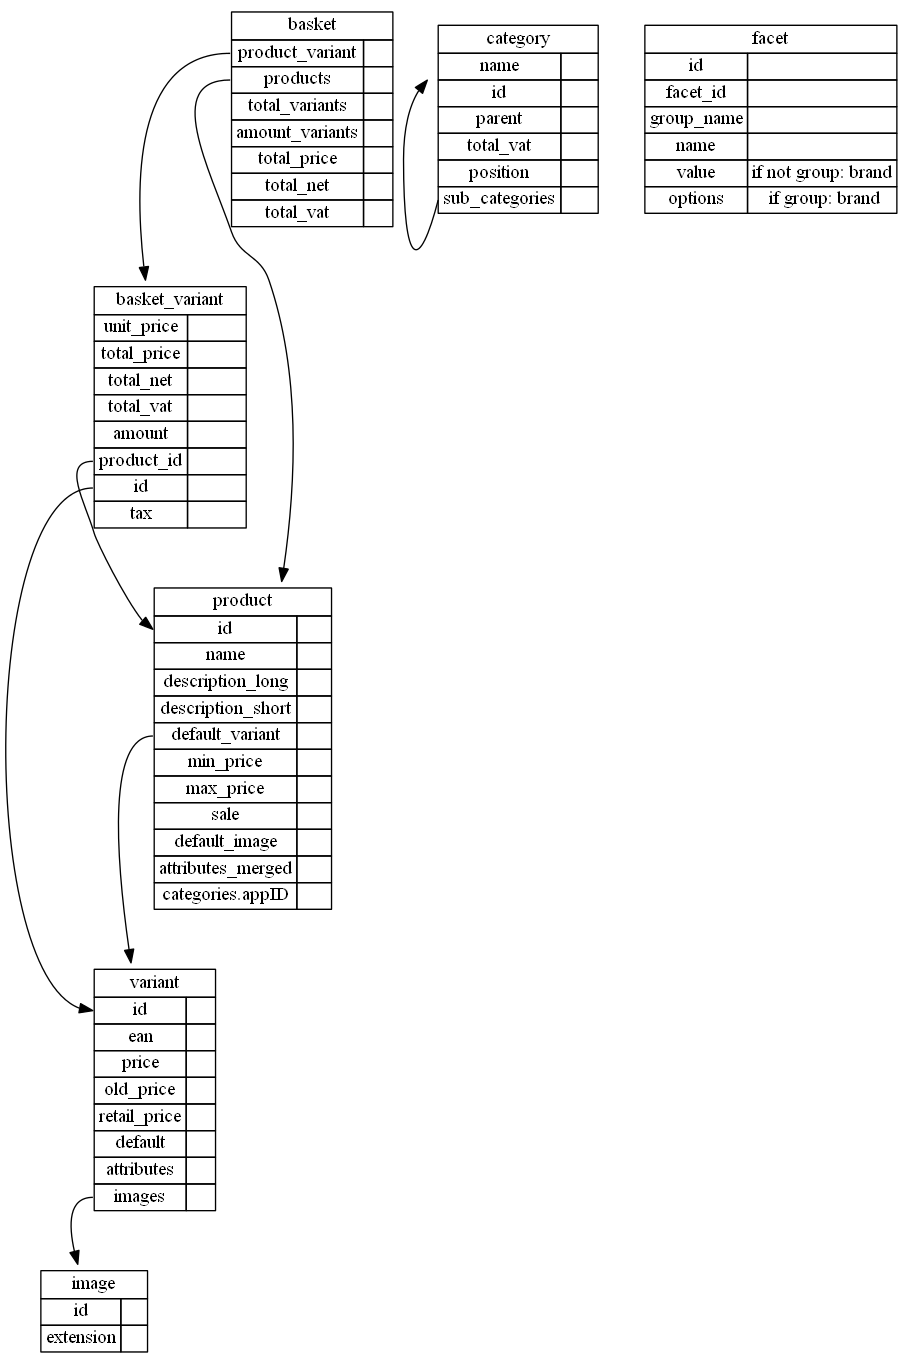
\includegraphics{collins_objects.png}
\index{COLLINS\_VERSION (in module collins)}

\begin{fulllineitems}
\phantomsection\label{collins:collins.COLLINS_VERSION}\pysigline{\code{collins.}\bfcode{COLLINS\_VERSION}\strong{ = `1.1'}}
The version of the collins api which is supported.

\end{fulllineitems}

\index{Collins (class in collins)}

\begin{fulllineitems}
\phantomsection\label{collins:collins.Collins}\pysiglinewithargsret{\strong{class }\code{collins.}\bfcode{Collins}}{\emph{config}}{}
Bases: \code{object}

An interface to the Collins API.

This is thin warper around the Collins API.
All functions return the JSON responses as Python List and Dictonarys.
\begin{quote}\begin{description}
\item[{Parameters}] \leavevmode
\textbf{config} -- A Config instance or a file name to a JSON config file.

\end{description}\end{quote}
\index{autocomplete() (collins.Collins method)}

\begin{fulllineitems}
\phantomsection\label{collins:collins.Collins.autocomplete}\pysiglinewithargsret{\bfcode{autocomplete}}{\emph{searchword}, \emph{limit=None}, \emph{types=None}}{}~\begin{quote}\begin{description}
\item[{Parameters}] \leavevmode\begin{itemize}
\item {} 
\textbf{searchword} (\emph{str}) -- The abbriviation.

\item {} 
\textbf{categories} (\emph{list}) -- against which types should be autocompleted

\item {} 
\textbf{limit} (\emph{int}) -- the amount of items returned per selected type

\end{itemize}

\end{description}\end{quote}

\begin{notice}{attention}{Attention:}
In the documentation stands \textbf{autocomplete} but the real
Tag is \textbf{autocompletion}!
\end{notice}

\end{fulllineitems}

\index{basketadd() (collins.Collins method)}

\begin{fulllineitems}
\phantomsection\label{collins:collins.Collins.basketadd}\pysiglinewithargsret{\bfcode{basketadd}}{\emph{sessionid}, \emph{products}}{}
The request ``basket add'' does change the Items available in the basket.
A set to 0 or less leads to a deletion. Only the variants in the items
list will be changed. If a variant is changed or added an internal
availability check is done and error codes are returned.
\begin{quote}\begin{description}
\item[{Parameters}] \leavevmode\begin{itemize}
\item {} 
\textbf{sessionid} (\emph{str}) -- identification of the basket -\textgreater{} user,
user -\textgreater{} basket

\item {} 
\textbf{products} (\emph{list}) -- is the array for the product variants

\end{itemize}

\end{description}\end{quote}
\paragraph{product variant dict}

\begin{tabulary}{\linewidth}{|L|L|}
\hline
\textsf{\relax 
fieldname
} & \textsf{\relax 
meaning
}\\
\hline
id
 & 
the product variant id
\\

command
 & 
either add for the + operator (even -1 is possible)
or set for a specific quantity.
If the end amount is \textless{}= 0 the product is
removed from basket with an result code.
\\

amount
 & 
the amount to add or set
\\
\hline\end{tabulary}


\end{fulllineitems}

\index{basketget() (collins.Collins method)}

\begin{fulllineitems}
\phantomsection\label{collins:collins.Collins.basketget}\pysiglinewithargsret{\bfcode{basketget}}{\emph{sessionid}}{}
This returns the current basket for a User / Session ID.
The basket belongs to a specific app id and session id,
another app can have the same session id.
\begin{quote}\begin{description}
\item[{Parameters}] \leavevmode
\textbf{sessionid} (\emph{str}) -- identification of the basket -\textgreater{} user,
user -\textgreater{} basket

\end{description}\end{quote}

\end{fulllineitems}

\index{category() (collins.Collins method)}

\begin{fulllineitems}
\phantomsection\label{collins:collins.Collins.category}\pysiglinewithargsret{\bfcode{category}}{\emph{ids}}{}
You are able to retrieve single categories.
\begin{quote}\begin{description}
\item[{Parameters}] \leavevmode
\textbf{ids} (\emph{list}) -- List of category ids.

\end{description}\end{quote}
\paragraph{Example}

\begin{Verbatim}[commandchars=\\\{\}]
\PYG{n}{collins}\PYG{o}{.}\PYG{n}{category}\PYG{p}{(}\PYG{p}{[}\PYG{l+m+mi}{16077}\PYG{p}{]}\PYG{p}{)}
\end{Verbatim}

\begin{Verbatim}[commandchars=\\\{\}]
\PYG{p}{\PYGZob{}}
    \PYG{n+nt}{\PYGZdq{}16077\PYGZdq{}}\PYG{p}{:} \PYG{p}{\PYGZob{}}
        \PYG{n+nt}{\PYGZdq{}active\PYGZdq{}}\PYG{p}{:} \PYG{k+kc}{true}\PYG{p}{,}
        \PYG{n+nt}{\PYGZdq{}position\PYGZdq{}}\PYG{p}{:} \PYG{l+m+mi}{1}\PYG{p}{,}
        \PYG{n+nt}{\PYGZdq{}name\PYGZdq{}}\PYG{p}{:} \PYG{l+s+s2}{\PYGZdq{}Damen\PYGZdq{}}\PYG{p}{,}
        \PYG{n+nt}{\PYGZdq{}parent\PYGZdq{}}\PYG{p}{:} \PYG{l+m+mi}{0}\PYG{p}{,}
        \PYG{n+nt}{\PYGZdq{}id\PYGZdq{}}\PYG{p}{:} \PYG{l+m+mi}{16077}
    \PYG{p}{\PYGZcb{}}
\PYG{p}{\PYGZcb{}}
\end{Verbatim}

\end{fulllineitems}

\index{categorytree() (collins.Collins method)}

\begin{fulllineitems}
\phantomsection\label{collins:collins.Collins.categorytree}\pysiglinewithargsret{\bfcode{categorytree}}{\emph{max\_depth=None}}{}
The request category tree returns a tree of categories of a
specified max depth for your app id.
\begin{quote}\begin{description}
\item[{Parameters}] \leavevmode
\textbf{max\_depth} (\emph{int}) -- max depth of your category tree counted from root

\end{description}\end{quote}
\paragraph{Example}

\begin{Verbatim}[commandchars=\\\{\}]
\PYG{n}{collins}\PYG{o}{.}\PYG{n}{categorytree}\PYG{p}{(}\PYG{p}{)}
\end{Verbatim}

\begin{Verbatim}[commandchars=\\\{\}]
\PYG{p}{[}
    \PYG{p}{\PYGZob{}}
        \PYG{n+nt}{\PYGZdq{}name\PYGZdq{}}\PYG{p}{:} \PYG{l+s+s2}{\PYGZdq{}Damen\PYGZdq{}}\PYG{p}{,}
        \PYG{n+nt}{\PYGZdq{}parent\PYGZdq{}}\PYG{p}{:} \PYG{k+kc}{null}\PYG{p}{,}
        \PYG{n+nt}{\PYGZdq{}sub\PYGZus{}categories\PYGZdq{}}\PYG{p}{:} \PYG{p}{[}
            \PYG{p}{\PYGZob{}}
                \PYG{n+nt}{\PYGZdq{}name\PYGZdq{}}\PYG{p}{:} \PYG{l+s+s2}{\PYGZdq{}Bekleidung\PYGZdq{}}\PYG{p}{,}
                \PYG{n+nt}{\PYGZdq{}parent\PYGZdq{}}\PYG{p}{:} \PYG{l+m+mi}{16077}\PYG{p}{,}
                \PYG{n+nt}{\PYGZdq{}sub\PYGZus{}categories\PYGZdq{}}\PYG{p}{:} \PYG{p}{[}
                    \PYG{p}{\PYGZob{}}
                        \PYG{n+nt}{\PYGZdq{}name\PYGZdq{}}\PYG{p}{:} \PYG{l+s+s2}{\PYGZdq{}Oberteile\PYGZdq{}}\PYG{p}{,}
                        \PYG{n+nt}{\PYGZdq{}parent\PYGZdq{}}\PYG{p}{:} \PYG{l+m+mi}{16078}\PYG{p}{,}
                        \PYG{n+nt}{\PYGZdq{}sub\PYGZus{}categories\PYGZdq{}}\PYG{p}{:} \PYG{p}{[}
                            \PYG{p}{\PYGZob{}}
                                \PYG{n+nt}{\PYGZdq{}name\PYGZdq{}}\PYG{p}{:} \PYG{l+s+s2}{\PYGZdq{}Fr\PYGZbs{}u00fchlingslooks\PYGZdq{}}\PYG{p}{,}
                                \PYG{n+nt}{\PYGZdq{}parent\PYGZdq{}}\PYG{p}{:} \PYG{l+m+mi}{16079}\PYG{p}{,}
                                \PYG{n+nt}{\PYGZdq{}sub\PYGZus{}categories\PYGZdq{}}\PYG{p}{:} \PYG{p}{[}\PYG{p}{]}\PYG{p}{,}
                                \PYG{n+nt}{\PYGZdq{}active\PYGZdq{}}\PYG{p}{:} \PYG{k+kc}{false}\PYG{p}{,}
                                \PYG{n+nt}{\PYGZdq{}position\PYGZdq{}}\PYG{p}{:} \PYG{l+m+mi}{1}\PYG{p}{,}
                                \PYG{n+nt}{\PYGZdq{}id\PYGZdq{}}\PYG{p}{:} \PYG{l+m+mi}{23882}
                            \PYG{p}{\PYGZcb{}}
                        \PYG{p}{]}
                    \PYG{p}{\PYGZcb{}}
                \PYG{p}{]}
            \PYG{p}{\PYGZcb{}}
        \PYG{p}{]}
    \PYG{p}{\PYGZcb{}}
\PYG{p}{]}
\end{Verbatim}

\end{fulllineitems}

\index{facets() (collins.Collins method)}

\begin{fulllineitems}
\phantomsection\label{collins:collins.Collins.facets}\pysiglinewithargsret{\bfcode{facets}}{\emph{group\_ids=None}, \emph{limit=None}, \emph{offset=None}}{}
This returns a list of available facet groups or a facets of a group.
\begin{quote}\begin{description}
\item[{Parameters}] \leavevmode\begin{itemize}
\item {} 
\textbf{group\_ids} (\emph{list}) -- get only these group ids, if empty get all
group ids which belong to me

\item {} 
\textbf{limit} (\emph{int}) -- limit the per page items

\item {} 
\textbf{offset} (\emph{int}) -- offset for paging through the items

\end{itemize}

\end{description}\end{quote}
\paragraph{Example}

\begin{Verbatim}[commandchars=\\\{\}]
\PYG{n}{collins}\PYG{o}{.}\PYG{n}{facets}\PYG{p}{(}\PYG{p}{[}\PYG{n}{Constants}\PYG{o}{.}\PYG{n}{FACET\PYGZus{}CUPSIZE}\PYG{p}{]}\PYG{p}{)}
\end{Verbatim}

\begin{Verbatim}[commandchars=\\\{\}]
\PYG{p}{\PYGZob{}}
    \PYG{n+nt}{\PYGZdq{}facet\PYGZdq{}}\PYG{p}{:} \PYG{p}{[}
        \PYG{p}{\PYGZob{}}
            \PYG{n+nt}{\PYGZdq{}id\PYGZdq{}}\PYG{p}{:} \PYG{l+m+mi}{4}\PYG{p}{,}
            \PYG{n+nt}{\PYGZdq{}group\PYGZus{}name\PYGZdq{}}\PYG{p}{:} \PYG{l+s+s2}{\PYGZdq{}cupsize\PYGZdq{}}\PYG{p}{,}
            \PYG{n+nt}{\PYGZdq{}name\PYGZdq{}}\PYG{p}{:} \PYG{l+s+s2}{\PYGZdq{}D\PYGZdq{}}\PYG{p}{,}
            \PYG{n+nt}{\PYGZdq{}value\PYGZdq{}}\PYG{p}{:} \PYG{l+s+s2}{\PYGZdq{}D\PYGZdq{}}\PYG{p}{,}
            \PYG{n+nt}{\PYGZdq{}facet\PYGZus{}id\PYGZdq{}}\PYG{p}{:} \PYG{l+m+mi}{96}
        \PYG{p}{\PYGZcb{}}\PYG{p}{,}
        \PYG{p}{\PYGZob{}}
            \PYG{n+nt}{\PYGZdq{}id\PYGZdq{}}\PYG{p}{:} \PYG{l+m+mi}{4}\PYG{p}{,}
            \PYG{n+nt}{\PYGZdq{}group\PYGZus{}name\PYGZdq{}}\PYG{p}{:} \PYG{l+s+s2}{\PYGZdq{}cupsize\PYGZdq{}}\PYG{p}{,}
            \PYG{n+nt}{\PYGZdq{}name\PYGZdq{}}\PYG{p}{:} \PYG{l+s+s2}{\PYGZdq{}A\PYGZdq{}}\PYG{p}{,}
            \PYG{n+nt}{\PYGZdq{}value\PYGZdq{}}\PYG{p}{:} \PYG{l+s+s2}{\PYGZdq{}A\PYGZdq{}}\PYG{p}{,}
            \PYG{n+nt}{\PYGZdq{}facet\PYGZus{}id\PYGZdq{}}\PYG{p}{:} \PYG{l+m+mi}{93}
        \PYG{p}{\PYGZcb{}}\PYG{p}{,}
        \PYG{p}{\PYGZob{}}
            \PYG{n+nt}{\PYGZdq{}id\PYGZdq{}}\PYG{p}{:} \PYG{l+m+mi}{4}\PYG{p}{,}
            \PYG{n+nt}{\PYGZdq{}group\PYGZus{}name\PYGZdq{}}\PYG{p}{:} \PYG{l+s+s2}{\PYGZdq{}cupsize\PYGZdq{}}\PYG{p}{,}
            \PYG{n+nt}{\PYGZdq{}name\PYGZdq{}}\PYG{p}{:} \PYG{l+s+s2}{\PYGZdq{}B\PYGZdq{}}\PYG{p}{,}
            \PYG{n+nt}{\PYGZdq{}value\PYGZdq{}}\PYG{p}{:} \PYG{l+s+s2}{\PYGZdq{}B\PYGZdq{}}\PYG{p}{,}
            \PYG{n+nt}{\PYGZdq{}facet\PYGZus{}id\PYGZdq{}}\PYG{p}{:} \PYG{l+m+mi}{94}
        \PYG{p}{\PYGZcb{}}\PYG{p}{,}
        \PYG{p}{\PYGZob{}}
            \PYG{n+nt}{\PYGZdq{}id\PYGZdq{}}\PYG{p}{:} \PYG{l+m+mi}{4}\PYG{p}{,}
            \PYG{n+nt}{\PYGZdq{}group\PYGZus{}name\PYGZdq{}}\PYG{p}{:} \PYG{l+s+s2}{\PYGZdq{}cupsize\PYGZdq{}}\PYG{p}{,}
            \PYG{n+nt}{\PYGZdq{}name\PYGZdq{}}\PYG{p}{:} \PYG{l+s+s2}{\PYGZdq{}C\PYGZdq{}}\PYG{p}{,}
            \PYG{n+nt}{\PYGZdq{}value\PYGZdq{}}\PYG{p}{:} \PYG{l+s+s2}{\PYGZdq{}C\PYGZdq{}}\PYG{p}{,}
            \PYG{n+nt}{\PYGZdq{}facet\PYGZus{}id\PYGZdq{}}\PYG{p}{:} \PYG{l+m+mi}{95}
        \PYG{p}{\PYGZcb{}}
    \PYG{p}{]}\PYG{p}{,}
    \PYG{n+nt}{\PYGZdq{}hits\PYGZdq{}}\PYG{p}{:} \PYG{l+m+mi}{4}
\PYG{p}{\PYGZcb{}}
\end{Verbatim}

\end{fulllineitems}

\index{facettypes() (collins.Collins method)}

\begin{fulllineitems}
\phantomsection\label{collins:collins.Collins.facettypes}\pysiglinewithargsret{\bfcode{facettypes}}{}{}
This query returns a list of facet groups available.
\paragraph{Example}

\begin{Verbatim}[commandchars=\\\{\}]
\PYG{n}{collins}\PYG{o}{.}\PYG{n}{facettypes}\PYG{p}{(}\PYG{p}{)}
\end{Verbatim}

\begin{Verbatim}[commandchars=\\\{\}]
\PYG{p}{[}\PYG{l+m+mi}{0}\PYG{p}{,} \PYG{l+m+mi}{2}\PYG{p}{,} \PYG{l+m+mi}{1}\PYG{p}{,} \PYG{l+m+mi}{6}\PYG{p}{,} \PYG{l+m+mi}{172}\PYG{p}{,} \PYG{l+m+mi}{206}\PYG{p}{,} \PYG{l+m+mi}{173}\PYG{p}{,} \PYG{l+m+mi}{194}\PYG{p}{,} \PYG{l+m+mi}{175}\PYG{p}{,} \PYG{l+m+mi}{204}\PYG{p}{,} \PYG{l+m+mi}{5}\PYG{p}{,} \PYG{l+m+mi}{189}\PYG{p}{,} \PYG{l+m+mi}{180}\PYG{p}{,} \PYG{l+m+mi}{231}\PYG{p}{,} \PYG{l+m+mi}{187}\PYG{p}{,} \PYG{l+m+mi}{190}\PYG{p}{,} \PYG{l+m+mi}{211}\PYG{p}{,} \PYG{l+m+mi}{181}\PYG{p}{,} \PYG{l+m+mi}{247}\PYG{p}{]}
\end{Verbatim}

\end{fulllineitems}

\index{getorder() (collins.Collins method)}

\begin{fulllineitems}
\phantomsection\label{collins:collins.Collins.getorder}\pysiglinewithargsret{\bfcode{getorder}}{\emph{orderid}}{}~\begin{description}
\item[{Through this query you could get a order which was created}] \leavevmode
for/through your app. This is limited to a configured
timeframe and to your app.

\end{description}
\begin{quote}\begin{description}
\item[{Parameters}] \leavevmode
\textbf{orderid} (\emph{int}) -- this is the order id to get info about

\end{description}\end{quote}

\end{fulllineitems}

\index{initiateorder() (collins.Collins method)}

\begin{fulllineitems}
\phantomsection\label{collins:collins.Collins.initiateorder}\pysiglinewithargsret{\bfcode{initiateorder}}{\emph{sessionid}, \emph{sucess\_url}, \emph{cancel\_url=None}, \emph{error\_url=None}}{}~\begin{description}
\item[{At this request you initiate a order to a basket.}] \leavevmode
This should be done if a user wants to go to the checkout.

\end{description}
\begin{quote}\begin{description}
\item[{Parameters}] \leavevmode\begin{itemize}
\item {} 
\textbf{sessionid} (\emph{str}) -- identification of the basket -\textgreater{} user,
user -\textgreater{} basket (see basket\_get, basket\_add)

\item {} 
\textbf{sucess\_url} (\emph{str}) -- this is a callback url if the order was
successfully created. (see checkout api)

\item {} 
\textbf{cancel\_url} (\emph{str}) -- this is a callback url if the order was
canceled. (see checkout api)

\item {} 
\textbf{error\_url} (\emph{str}) -- this is a callback url if the order throwed
exceptions (see checkout api)

\end{itemize}

\end{description}\end{quote}

\end{fulllineitems}

\index{livevariant() (collins.Collins method)}

\begin{fulllineitems}
\phantomsection\label{collins:collins.Collins.livevariant}\pysiglinewithargsret{\bfcode{livevariant}}{\emph{ids}}{}~\begin{description}
\item[{This does return the live information about the product variant.}] \leavevmode
This is as ``live'' as possible.
And could differ vs. a ``product search'' or ``product'' query.

\end{description}
\begin{quote}\begin{description}
\item[{Parameters}] \leavevmode
\textbf{ids} (\emph{list}) -- array of product variant id

\end{description}\end{quote}

\end{fulllineitems}

\index{products() (collins.Collins method)}

\begin{fulllineitems}
\phantomsection\label{collins:collins.Collins.products}\pysiglinewithargsret{\bfcode{products}}{\emph{ids}, \emph{fields=None}}{}
Here you get a detail view of a product or a list of products returned
by its ids.
\begin{quote}\begin{description}
\item[{Parameters}] \leavevmode
\textbf{ids} (\emph{list}) -- array of product variant id

\end{description}\end{quote}
\paragraph{Example}

\begin{Verbatim}[commandchars=\\\{\}]
\PYG{n}{collins}\PYG{o}{.}\PYG{n}{products}\PYG{p}{(}\PYG{p}{[}\PYG{l+m+mi}{227838}\PYG{p}{,} \PYG{l+m+mi}{287677}\PYG{p}{]}\PYG{p}{)}
\end{Verbatim}

\begin{Verbatim}[commandchars=\\\{\}]
\PYG{p}{\PYGZob{}}
    \PYG{n+nt}{\PYGZdq{}pageHash\PYGZdq{}}\PYG{p}{:} \PYG{l+s+s2}{\PYGZdq{}4ae38022\PYGZhy{}8ddd\PYGZhy{}4f15\PYGZhy{}9654\PYGZhy{}4ea0156c33f0\PYGZdq{}}\PYG{p}{,}
    \PYG{n+nt}{\PYGZdq{}ids\PYGZdq{}}\PYG{p}{:} \PYG{p}{\PYGZob{}}
        \PYG{n+nt}{\PYGZdq{}287677\PYGZdq{}}\PYG{p}{:} \PYG{p}{\PYGZob{}}
            \PYG{n+nt}{\PYGZdq{}active\PYGZdq{}}\PYG{p}{:} \PYG{k+kc}{true}\PYG{p}{,}
            \PYG{n+nt}{\PYGZdq{}styles\PYGZdq{}}\PYG{p}{:} \PYG{p}{[}
                \PYG{p}{\PYGZob{}}
                    \PYG{n+nt}{\PYGZdq{}active\PYGZdq{}}\PYG{p}{:} \PYG{k+kc}{true}\PYG{p}{,}
                    \PYG{n+nt}{\PYGZdq{}id\PYGZdq{}}\PYG{p}{:} \PYG{l+m+mi}{287685}\PYG{p}{,}
                    \PYG{n+nt}{\PYGZdq{}style\PYGZus{}key\PYGZdq{}}\PYG{p}{:} \PYG{l+s+s2}{\PYGZdq{}m01\PYGZus{}233966406\PYGZdq{}}\PYG{p}{,}
                    \PYG{n+nt}{\PYGZdq{}name\PYGZdq{}}\PYG{p}{:} \PYG{l+s+s2}{\PYGZdq{}Badeshorts, Buffalo\PYGZdq{}}
                \PYG{p}{\PYGZcb{}}\PYG{p}{,}
                \PYG{p}{\PYGZob{}}
                    \PYG{n+nt}{\PYGZdq{}active\PYGZdq{}}\PYG{p}{:} \PYG{k+kc}{false}\PYG{p}{,}
                    \PYG{n+nt}{\PYGZdq{}id\PYGZdq{}}\PYG{p}{:} \PYG{l+m+mi}{358863}\PYG{p}{,}
                    \PYG{n+nt}{\PYGZdq{}style\PYGZus{}key\PYGZdq{}}\PYG{p}{:} \PYG{l+s+s2}{\PYGZdq{}m01\PYGZus{}233966406\PYGZdq{}}\PYG{p}{,}
                    \PYG{n+nt}{\PYGZdq{}name\PYGZdq{}}\PYG{p}{:} \PYG{l+s+s2}{\PYGZdq{}Badeshorts, Buffalo\PYGZdq{}}
                \PYG{p}{\PYGZcb{}}
            \PYG{p}{]}\PYG{p}{,}
            \PYG{n+nt}{\PYGZdq{}id\PYGZdq{}}\PYG{p}{:} \PYG{l+m+mi}{287677}\PYG{p}{,}
            \PYG{n+nt}{\PYGZdq{}style\PYGZus{}key\PYGZdq{}}\PYG{p}{:} \PYG{l+s+s2}{\PYGZdq{}m01\PYGZus{}233966406\PYGZdq{}}\PYG{p}{,}
            \PYG{n+nt}{\PYGZdq{}name\PYGZdq{}}\PYG{p}{:} \PYG{l+s+s2}{\PYGZdq{}Badeshorts, Buffalo\PYGZdq{}}
        \PYG{p}{\PYGZcb{}}\PYG{p}{,}
        \PYG{n+nt}{\PYGZdq{}227838\PYGZdq{}}\PYG{p}{:} \PYG{p}{\PYGZob{}}
            \PYG{n+nt}{\PYGZdq{}active\PYGZdq{}}\PYG{p}{:} \PYG{k+kc}{true}\PYG{p}{,}
            \PYG{n+nt}{\PYGZdq{}styles\PYGZdq{}}\PYG{p}{:} \PYG{p}{[}
                \PYG{p}{\PYGZob{}}
                    \PYG{n+nt}{\PYGZdq{}active\PYGZdq{}}\PYG{p}{:} \PYG{k+kc}{true}\PYG{p}{,}
                    \PYG{n+nt}{\PYGZdq{}id\PYGZdq{}}\PYG{p}{:} \PYG{l+m+mi}{227854}\PYG{p}{,}
                    \PYG{n+nt}{\PYGZdq{}style\PYGZus{}key\PYGZdq{}}\PYG{p}{:} \PYG{l+s+s2}{\PYGZdq{}m01\PYGZus{}255897631\PYGZdq{}}\PYG{p}{,}
                    \PYG{n+nt}{\PYGZdq{}name\PYGZdq{}}\PYG{p}{:} \PYG{l+s+s2}{\PYGZdq{}Badeshort Herren\PYGZdq{}}
                \PYG{p}{\PYGZcb{}}
            \PYG{p}{]}\PYG{p}{,}
            \PYG{n+nt}{\PYGZdq{}id\PYGZdq{}}\PYG{p}{:} \PYG{l+m+mi}{227838}\PYG{p}{,}
            \PYG{n+nt}{\PYGZdq{}style\PYGZus{}key\PYGZdq{}}\PYG{p}{:} \PYG{l+s+s2}{\PYGZdq{}m01\PYGZus{}255897631\PYGZdq{}}\PYG{p}{,}
            \PYG{n+nt}{\PYGZdq{}name\PYGZdq{}}\PYG{p}{:} \PYG{l+s+s2}{\PYGZdq{}Badeshort Herren\PYGZdq{}}
        \PYG{p}{\PYGZcb{}}
    \PYG{p}{\PYGZcb{}}
\PYG{p}{\PYGZcb{}}
\end{Verbatim}

\end{fulllineitems}

\index{productsearch() (collins.Collins method)}

\begin{fulllineitems}
\phantomsection\label{collins:collins.Collins.productsearch}\pysiglinewithargsret{\bfcode{productsearch}}{\emph{sessionid}, \emph{filter=None}, \emph{result=None}}{}
This is the main query for retrieving products for your app.
Lists of products will be returned which are filtered.
In a search you dont get back inactive set products.
The response can contain the available facets and their product count
and categories for the filter set.
\begin{description}
\item[{There are two types of facets:}] \leavevmode\begin{enumerate}
\item {} \begin{description}
\item[{is a pre defined and always available set of facets}] \leavevmode\begin{enumerate}
\item {} 
price range (amazon like see )

\item {} 
sale facet how many products are sale and how many not

\item {} 
categories

\end{enumerate}

\end{description}

\item {} 
dynamic facets which occur through the products itself. If a
product has one the these attributes you are able to query for
these attributes. These facets are always just ids.
The name -\textgreater{} id, id -\textgreater{} name resolution works through facets call.
To get all the facet groups you can filter or are in your result
set see ``Facet types''

\end{enumerate}

\end{description}

\begin{notice}{note}{Note:}
To get facet types see {\hyperref[collins:collins.Constants]{\code{collins.Constants}}}
\end{notice}
\begin{quote}\begin{description}
\item[{Parameters}] \leavevmode\begin{itemize}
\item {} 
\textbf{sessionid} (\emph{str}) -- the session\_id of the frontend customer

\item {} 
\textbf{filter} (\emph{dict}) -- object of filter information, these filters do
change the subset of products

\item {} 
\textbf{result} (\emph{dict}) -- object of result information, these properties
change the order and the appearance of the subset

\end{itemize}

\end{description}\end{quote}
\paragraph{filter dict}

\begin{tabulary}{\linewidth}{|L|L|}
\hline
\textsf{\relax 
fieldname
} & \textsf{\relax 
meaning
}\\
\hline
categories
 & 
array of category ids to include the products from
\\

sale
 & 
true =\textgreater{} only sale products
false =\textgreater{} no sale products
null =\textgreater{} both
\\

prices
 & 
is an object with properties from and to which lead to
range filter on the price set as eurocent
\\

searchword
 & 
the word which filters every product
\\

facets
 & 
object of attributes every key is an array of facet id
values to filter by them
\\
\hline\end{tabulary}

\paragraph{result dict}

\begin{tabulary}{\linewidth}{|L|L|}
\hline
\textsf{\relax 
fieldname
} & \textsf{\relax 
meaning
}\\
\hline
sort
 & 
how to sort the products
\\

price
 & 
geta back a range of attributes and their product counts
also some statistical information in eurocent.
\\

sale
 & 
product count of products which are in sale
\\

facets
 & 
object of which facet get back what count of facets
\\

categories
 & 
set if get or not back the categories in which are products
and the count of products
\\

limit
 & 
how many products to get back
\\

offset
 & 
the offset where to start to get the products from
\\
\hline\end{tabulary}

\paragraph{result.facets dict}

\begin{tabulary}{\linewidth}{|L|L|}
\hline
\textsf{\relax 
fieldname
} & \textsf{\relax 
meaning
}\\
\hline
\_all
 & 
is an object with property limit which holds an integer
to get the amount of attributes, sort by occurrences in
products if this is set, this is the default for
ALL attributes.
\\

{[} 0-9 {]}+
 & 
is an object with property limit which holds an integer to
get the amount of attributes of this attribute group id,
sort by occurrences in products. this overwrites even the
\_all field.
\\
\hline\end{tabulary}

\paragraph{Example}

\begin{Verbatim}[commandchars=\\\{\}]
\PYG{c}{\PYGZsh{} i belive we search shorts now o.O}
\PYG{n}{collins}\PYG{o}{.}\PYG{n}{productsearch}\PYG{p}{(}\PYG{n}{TEST\PYGZus{}SESSION\PYGZus{}ID}\PYG{p}{,} \PYG{n+nb}{filter}\PYG{o}{=}\PYG{p}{\PYGZob{}}\PYG{l+s}{\PYGZdq{}}\PYG{l+s}{categories}\PYG{l+s}{\PYGZdq{}}\PYG{p}{:}\PYG{p}{[}\PYG{l+m+mi}{16354}\PYG{p}{]}\PYG{p}{\PYGZcb{}}\PYG{p}{)}
\end{Verbatim}

\begin{Verbatim}[commandchars=\\\{\}]
\PYG{p}{\PYGZob{}}
    \PYG{n+nt}{\PYGZdq{}product\PYGZus{}count\PYGZdq{}}\PYG{p}{:} \PYG{l+m+mi}{78}\PYG{p}{,}
    \PYG{n+nt}{\PYGZdq{}pageHash\PYGZdq{}}\PYG{p}{:} \PYG{l+s+s2}{\PYGZdq{}6e63cadb\PYGZhy{}5505\PYGZhy{}47b7\PYGZhy{}b36d\PYGZhy{}643311292a22\PYGZdq{}}\PYG{p}{,}
    \PYG{n+nt}{\PYGZdq{}facets\PYGZdq{}}\PYG{p}{:} \PYG{p}{\PYGZob{}}\PYG{p}{\PYGZcb{}}\PYG{p}{,}
    \PYG{n+nt}{\PYGZdq{}products\PYGZdq{}}\PYG{p}{:} \PYG{p}{[}
        \PYG{p}{\PYGZob{}}
            \PYG{n+nt}{\PYGZdq{}id\PYGZdq{}}\PYG{p}{:} \PYG{l+m+mi}{227838}\PYG{p}{,}
            \PYG{n+nt}{\PYGZdq{}name\PYGZdq{}}\PYG{p}{:} \PYG{l+s+s2}{\PYGZdq{}Badeshort Herren\PYGZdq{}}
        \PYG{p}{\PYGZcb{}}
    \PYG{p}{]}
\PYG{p}{\PYGZcb{}}
\end{Verbatim}

\end{fulllineitems}

\index{send() (collins.Collins method)}

\begin{fulllineitems}
\phantomsection\label{collins:collins.Collins.send}\pysiglinewithargsret{\bfcode{send}}{\emph{cmd}, \emph{obj}}{}
Sends a Pyhton structure of dict's and list's as raw JSON to collins and
returns a Python structure of dict's and list's from the JSON answer.
\begin{quote}\begin{description}
\item[{Parameters}] \leavevmode\begin{itemize}
\item {} 
\textbf{cmd} -- The name of the command.

\item {} 
\textbf{obj} -- A python dict object which contains the request parameters.

\end{itemize}

\end{description}\end{quote}

\end{fulllineitems}

\index{suggest() (collins.Collins method)}

\begin{fulllineitems}
\phantomsection\label{collins:collins.Collins.suggest}\pysiglinewithargsret{\bfcode{suggest}}{\emph{searchword}, \emph{categories=None}, \emph{limit=None}}{}
The suggest endpoint does what it says and suggest more terms.
It takes a searchterm and suggests terms which occurance is really
often in combination with these terms before.
\begin{quote}\begin{description}
\item[{Parameters}] \leavevmode\begin{itemize}
\item {} 
\textbf{searchword} (\emph{str}) -- string of a searchterm to suggest more words for

\item {} 
\textbf{categories} (\emph{list}) -- array of category ids

\item {} 
\textbf{limit} (\emph{int}) -- amount of items to suggest

\end{itemize}

\end{description}\end{quote}

\end{fulllineitems}


\end{fulllineitems}

\index{CollinsException}

\begin{fulllineitems}
\phantomsection\label{collins:collins.CollinsException}\pysigline{\strong{exception }\code{collins.}\bfcode{CollinsException}}
Bases: \code{exceptions.Exception}

An exception in the collins module.

\end{fulllineitems}

\index{Config (class in collins)}

\begin{fulllineitems}
\phantomsection\label{collins:collins.Config}\pysiglinewithargsret{\strong{class }\code{collins.}\bfcode{Config}}{\emph{filename}}{}
Bases: \code{object}

The configuration of a collins api connection.

A config class has to have the following readable attributes:
\begin{itemize}
\item {} \begin{description}
\item[{entry\_point\_url:}] \leavevmode
The url for collins.

\end{description}

\item {} \begin{description}
\item[{app\_id}] \leavevmode
The application id.

\end{description}

\item {} \begin{description}
\item[{app\_password}] \leavevmode
The password for the corresponding application id.

\end{description}

\item {} \begin{description}
\item[{agent}] \leavevmode
The name of the browser agent to fake.

\end{description}

\item {} \begin{description}
\item[{authorization}] \leavevmode
The authorization header

\end{description}

\item {} \begin{description}
\item[{image\_url}] \leavevmode
A string as template for the image urls.
As example \href{http://cdn.mary-paul.de/product\_images}{http://cdn.mary-paul.de/product\_images}/\{path\}/\{id\}\_\{width\}\_\{height\}\{extension\}.

\end{description}

\item {} \begin{description}
\item[{logging}] \leavevmode
A dictonary for logging.config.dictConfig.

\end{description}

\end{itemize}
\begin{quote}\begin{description}
\item[{Parameters}] \leavevmode
\textbf{filename} (\emph{str}) -- The path to a JSON file which holds the configuration.

\end{description}\end{quote}
\index{imageurl() (collins.Config method)}

\begin{fulllineitems}
\phantomsection\label{collins:collins.Config.imageurl}\pysiglinewithargsret{\bfcode{imageurl}}{\emph{path}, \emph{productid}, \emph{width}, \emph{height}, \emph{extension}}{}
Returns the url for a image.
\begin{quote}\begin{description}
\item[{Parameters}] \leavevmode\begin{itemize}
\item {} 
\textbf{path} -- Part of the image path.

\item {} 
\textbf{productid} -- 

\item {} 
\textbf{width} -- Width of the image.

\item {} 
\textbf{height} -- Height of the image.

\item {} 
\textbf{extension} -- The image extension. For example \emph{`.jpg'}

\end{itemize}

\end{description}\end{quote}

\end{fulllineitems}


\end{fulllineitems}

\index{Constants (class in collins)}

\begin{fulllineitems}
\phantomsection\label{collins:collins.Constants}\pysigline{\strong{class }\code{collins.}\bfcode{Constants}}
Bases: \code{object}

Some contsants which are blatantly copied from the php-sdk.

\begin{notice}{attention}{Attention:}\begin{description}
\item[{The following constants are \textbf{NOT} in the PHP-SDK:}] \leavevmode\begin{itemize}
\item {} 
FACET\_CHANNEL

\item {} 
FACET\_CARE\_SYMBOL

\item {} 
FACET\_CLOTHING\_HATS\_US

\end{itemize}

\end{description}
\end{notice}
\index{API\_ENVIRONMENT\_LIVE (collins.Constants attribute)}

\begin{fulllineitems}
\phantomsection\label{collins:collins.Constants.API_ENVIRONMENT_LIVE}\pysigline{\bfcode{API\_ENVIRONMENT\_LIVE}\strong{ = `live'}}
\end{fulllineitems}

\index{API\_ENVIRONMENT\_STAGE (collins.Constants attribute)}

\begin{fulllineitems}
\phantomsection\label{collins:collins.Constants.API_ENVIRONMENT_STAGE}\pysigline{\bfcode{API\_ENVIRONMENT\_STAGE}\strong{ = `stage'}}
\end{fulllineitems}

\index{FACETS (collins.Constants attribute)}

\begin{fulllineitems}
\phantomsection\label{collins:collins.Constants.FACETS}\pysigline{\bfcode{FACETS}\strong{ = set({[}0, 1, 194, 3, 4, 5, 6, 172, 2, 204, 173, 174, 175, 206, 195, 180, 181, 187, 189, 190{]})}}
\end{fulllineitems}

\index{FACET\_BRAND (collins.Constants attribute)}

\begin{fulllineitems}
\phantomsection\label{collins:collins.Constants.FACET_BRAND}\pysigline{\bfcode{FACET\_BRAND}\strong{ = 0}}
\end{fulllineitems}

\index{FACET\_CARE\_SYMBOL (collins.Constants attribute)}

\begin{fulllineitems}
\phantomsection\label{collins:collins.Constants.FACET_CARE_SYMBOL}\pysigline{\bfcode{FACET\_CARE\_SYMBOL}\strong{ = 247}}
\end{fulllineitems}

\index{FACET\_CHANNEL (collins.Constants attribute)}

\begin{fulllineitems}
\phantomsection\label{collins:collins.Constants.FACET_CHANNEL}\pysigline{\bfcode{FACET\_CHANNEL}\strong{ = 211}}
\end{fulllineitems}

\index{FACET\_CLOTHING\_HATS\_US (collins.Constants attribute)}

\begin{fulllineitems}
\phantomsection\label{collins:collins.Constants.FACET_CLOTHING_HATS_US}\pysigline{\bfcode{FACET\_CLOTHING\_HATS\_US}\strong{ = 231}}
\end{fulllineitems}

\index{FACET\_CLOTHING\_MEN\_BELTS\_CM (collins.Constants attribute)}

\begin{fulllineitems}
\phantomsection\label{collins:collins.Constants.FACET_CLOTHING_MEN_BELTS_CM}\pysigline{\bfcode{FACET\_CLOTHING\_MEN\_BELTS\_CM}\strong{ = 190}}
\end{fulllineitems}

\index{FACET\_CLOTHING\_MEN\_DE (collins.Constants attribute)}

\begin{fulllineitems}
\phantomsection\label{collins:collins.Constants.FACET_CLOTHING_MEN_DE}\pysigline{\bfcode{FACET\_CLOTHING\_MEN\_DE}\strong{ = 187}}
\end{fulllineitems}

\index{FACET\_CLOTHING\_MEN\_INCH (collins.Constants attribute)}

\begin{fulllineitems}
\phantomsection\label{collins:collins.Constants.FACET_CLOTHING_MEN_INCH}\pysigline{\bfcode{FACET\_CLOTHING\_MEN\_INCH}\strong{ = 189}}
\end{fulllineitems}

\index{FACET\_CLOTHING\_UNISEX\_INCH (collins.Constants attribute)}

\begin{fulllineitems}
\phantomsection\label{collins:collins.Constants.FACET_CLOTHING_UNISEX_INCH}\pysigline{\bfcode{FACET\_CLOTHING\_UNISEX\_INCH}\strong{ = 174}}
\end{fulllineitems}

\index{FACET\_CLOTHING\_UNISEX\_INT (collins.Constants attribute)}

\begin{fulllineitems}
\phantomsection\label{collins:collins.Constants.FACET_CLOTHING_UNISEX_INT}\pysigline{\bfcode{FACET\_CLOTHING\_UNISEX\_INT}\strong{ = 173}}
\end{fulllineitems}

\index{FACET\_CLOTHING\_UNISEX\_ONESIZE (collins.Constants attribute)}

\begin{fulllineitems}
\phantomsection\label{collins:collins.Constants.FACET_CLOTHING_UNISEX_ONESIZE}\pysigline{\bfcode{FACET\_CLOTHING\_UNISEX\_ONESIZE}\strong{ = 204}}
\end{fulllineitems}

\index{FACET\_CLOTHING\_WOMEN\_BELTS\_CM (collins.Constants attribute)}

\begin{fulllineitems}
\phantomsection\label{collins:collins.Constants.FACET_CLOTHING_WOMEN_BELTS_CM}\pysigline{\bfcode{FACET\_CLOTHING\_WOMEN\_BELTS\_CM}\strong{ = 181}}
\end{fulllineitems}

\index{FACET\_CLOTHING\_WOMEN\_DE (collins.Constants attribute)}

\begin{fulllineitems}
\phantomsection\label{collins:collins.Constants.FACET_CLOTHING_WOMEN_DE}\pysigline{\bfcode{FACET\_CLOTHING\_WOMEN\_DE}\strong{ = 175}}
\end{fulllineitems}

\index{FACET\_CLOTHING\_WOMEN\_INCH (collins.Constants attribute)}

\begin{fulllineitems}
\phantomsection\label{collins:collins.Constants.FACET_CLOTHING_WOMEN_INCH}\pysigline{\bfcode{FACET\_CLOTHING\_WOMEN\_INCH}\strong{ = 180}}
\end{fulllineitems}

\index{FACET\_COLOR (collins.Constants attribute)}

\begin{fulllineitems}
\phantomsection\label{collins:collins.Constants.FACET_COLOR}\pysigline{\bfcode{FACET\_COLOR}\strong{ = 1}}
\end{fulllineitems}

\index{FACET\_CUPSIZE (collins.Constants attribute)}

\begin{fulllineitems}
\phantomsection\label{collins:collins.Constants.FACET_CUPSIZE}\pysigline{\bfcode{FACET\_CUPSIZE}\strong{ = 4}}
\end{fulllineitems}

\index{FACET\_DIMENSION3 (collins.Constants attribute)}

\begin{fulllineitems}
\phantomsection\label{collins:collins.Constants.FACET_DIMENSION3}\pysigline{\bfcode{FACET\_DIMENSION3}\strong{ = 6}}
\end{fulllineitems}

\index{FACET\_GENDERAGE (collins.Constants attribute)}

\begin{fulllineitems}
\phantomsection\label{collins:collins.Constants.FACET_GENDERAGE}\pysigline{\bfcode{FACET\_GENDERAGE}\strong{ = 3}}
\end{fulllineitems}

\index{FACET\_LENGTH (collins.Constants attribute)}

\begin{fulllineitems}
\phantomsection\label{collins:collins.Constants.FACET_LENGTH}\pysigline{\bfcode{FACET\_LENGTH}\strong{ = 5}}
\end{fulllineitems}

\index{FACET\_SHOES\_UNISEX\_ADIDAS\_EUR (collins.Constants attribute)}

\begin{fulllineitems}
\phantomsection\label{collins:collins.Constants.FACET_SHOES_UNISEX_ADIDAS_EUR}\pysigline{\bfcode{FACET\_SHOES\_UNISEX\_ADIDAS\_EUR}\strong{ = 195}}
\end{fulllineitems}

\index{FACET\_SHOES\_UNISEX\_EUR (collins.Constants attribute)}

\begin{fulllineitems}
\phantomsection\label{collins:collins.Constants.FACET_SHOES_UNISEX_EUR}\pysigline{\bfcode{FACET\_SHOES\_UNISEX\_EUR}\strong{ = 194}}
\end{fulllineitems}

\index{FACET\_SIZE (collins.Constants attribute)}

\begin{fulllineitems}
\phantomsection\label{collins:collins.Constants.FACET_SIZE}\pysigline{\bfcode{FACET\_SIZE}\strong{ = 2}}
\end{fulllineitems}

\index{FACET\_SIZE\_CODE (collins.Constants attribute)}

\begin{fulllineitems}
\phantomsection\label{collins:collins.Constants.FACET_SIZE_CODE}\pysigline{\bfcode{FACET\_SIZE\_CODE}\strong{ = 206}}
\end{fulllineitems}

\index{FACET\_SIZE\_RUN (collins.Constants attribute)}

\begin{fulllineitems}
\phantomsection\label{collins:collins.Constants.FACET_SIZE_RUN}\pysigline{\bfcode{FACET\_SIZE\_RUN}\strong{ = 172}}
\end{fulllineitems}

\index{SORTS (collins.Constants attribute)}

\begin{fulllineitems}
\phantomsection\label{collins:collins.Constants.SORTS}\pysigline{\bfcode{SORTS}\strong{ = set({[}'relevance', `updated\_date', `price', `most\_viewed', `created\_date'{]})}}
\end{fulllineitems}

\index{SORT\_CREATED (collins.Constants attribute)}

\begin{fulllineitems}
\phantomsection\label{collins:collins.Constants.SORT_CREATED}\pysigline{\bfcode{SORT\_CREATED}\strong{ = `created\_date'}}
\end{fulllineitems}

\index{SORT\_MOST\_VIEWED (collins.Constants attribute)}

\begin{fulllineitems}
\phantomsection\label{collins:collins.Constants.SORT_MOST_VIEWED}\pysigline{\bfcode{SORT\_MOST\_VIEWED}\strong{ = `most\_viewed'}}
\end{fulllineitems}

\index{SORT\_PRICE (collins.Constants attribute)}

\begin{fulllineitems}
\phantomsection\label{collins:collins.Constants.SORT_PRICE}\pysigline{\bfcode{SORT\_PRICE}\strong{ = `price'}}
\end{fulllineitems}

\index{SORT\_RELEVANCE (collins.Constants attribute)}

\begin{fulllineitems}
\phantomsection\label{collins:collins.Constants.SORT_RELEVANCE}\pysigline{\bfcode{SORT\_RELEVANCE}\strong{ = `relevance'}}
\end{fulllineitems}

\index{SORT\_UPDATED (collins.Constants attribute)}

\begin{fulllineitems}
\phantomsection\label{collins:collins.Constants.SORT_UPDATED}\pysigline{\bfcode{SORT\_UPDATED}\strong{ = `updated\_date'}}
\end{fulllineitems}

\index{TYPES (collins.Constants attribute)}

\begin{fulllineitems}
\phantomsection\label{collins:collins.Constants.TYPES}\pysigline{\bfcode{TYPES}\strong{ = set({[}'products', `categories'{]})}}
\end{fulllineitems}

\index{TYPE\_CATEGORIES (collins.Constants attribute)}

\begin{fulllineitems}
\phantomsection\label{collins:collins.Constants.TYPE_CATEGORIES}\pysigline{\bfcode{TYPE\_CATEGORIES}\strong{ = `categories'}}
\end{fulllineitems}

\index{TYPE\_PRODUCTS (collins.Constants attribute)}

\begin{fulllineitems}
\phantomsection\label{collins:collins.Constants.TYPE_PRODUCTS}\pysigline{\bfcode{TYPE\_PRODUCTS}\strong{ = `products'}}
\end{fulllineitems}


\end{fulllineitems}

\index{EasyCollins (class in collins)}

\begin{fulllineitems}
\phantomsection\label{collins:collins.EasyCollins}\pysiglinewithargsret{\strong{class }\code{collins.}\bfcode{EasyCollins}}{\emph{conf\_or\_filename}}{}
Bases: \code{object}

\end{fulllineitems}

\index{VERSION (in module collins)}

\begin{fulllineitems}
\phantomsection\label{collins:collins.VERSION}\pysigline{\code{collins.}\bfcode{VERSION}\strong{ = `0.0'}}
Version of the python shop SDK.

\end{fulllineitems}

\index{check\_sessionid() (in module collins)}

\begin{fulllineitems}
\phantomsection\label{collins:collins.check_sessionid}\pysiglinewithargsret{\code{collins.}\bfcode{check\_sessionid}}{\emph{sessionid}}{}~
\begin{notice}{attention}{Attention:}
We copied it from the php-sdk.
collins seems to want have the session-id a minimum length of five
characters. This is not tested or validated.
\end{notice}

\end{fulllineitems}



\chapter{Indices and tables}
\label{index:indices-and-tables}\begin{itemize}
\item {} 
\emph{genindex}

\item {} 
\emph{modindex}

\item {} 
\emph{search}

\end{itemize}


\renewcommand{\indexname}{Python Module Index}
\begin{theindex}
\def\bigletter#1{{\Large\sffamily#1}\nopagebreak\vspace{1mm}}
\bigletter{c}
\item {\texttt{collins}}, \pageref{collins:module-collins}
\end{theindex}

\renewcommand{\indexname}{Index}
\printindex
\end{document}
